\chapter{Experimental Setup}\label{chapter:second_real_chapter}

\section{Implementation details}
\subsection{Dataset}
\paragraph{COCO~\cite{lin2015microsoftcococommonobjects}} is a publicly available dataset and has a multitude of labels. The semantic masks are extracted from the 2017 Panoptic annotations. This set contains more than 100k images that are densely annotated with both the semantic class and instance. There are a total of 133 different classes which belong to 27 `supercategories'. The four categories ``food'' and ``food-stuff'' and ``furniture'' and ``furniture-stuff'' were merged into ``food'' and ``furniture'' respectively, bringing the number of supercategories to 25. To speed up convergences, we will use these 25 classes. The distribution of the class labels can be seen in Figure \ref{fig:coco-class-distribution}. Some samples of the dataset can be seen in Figure \ref{fig:coco-samples}. More samples can be found in Appendix \ref{appendix:coco_samples}. 


\begin{figure}[h]
    \centering
    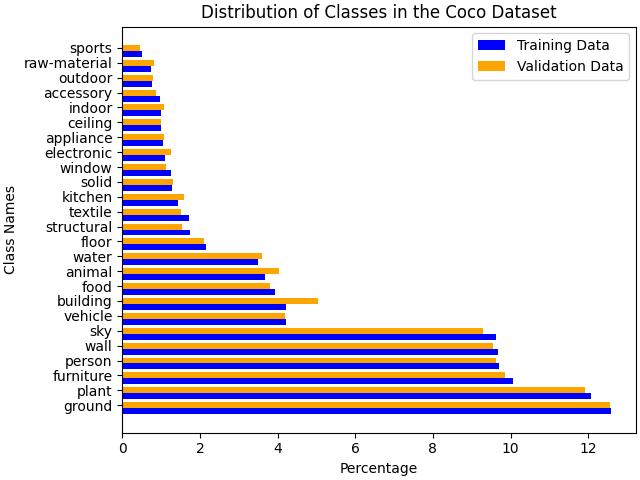
\includegraphics[width=0.9\textwidth]{figures/datasets/coco/class_distribution.png}
    \caption{Class Distribution of CoCo}
    \label{fig:coco-class-distribution}
\end{figure}

\begin{figure}
    \centering
    \subfloat[Training sample 0]{%
        
\includegraphics[width=0.5\textwidth]{figures/datasets/coco/samples/train/0.png}%
    }
    \subfloat[Training sample 1]{%
        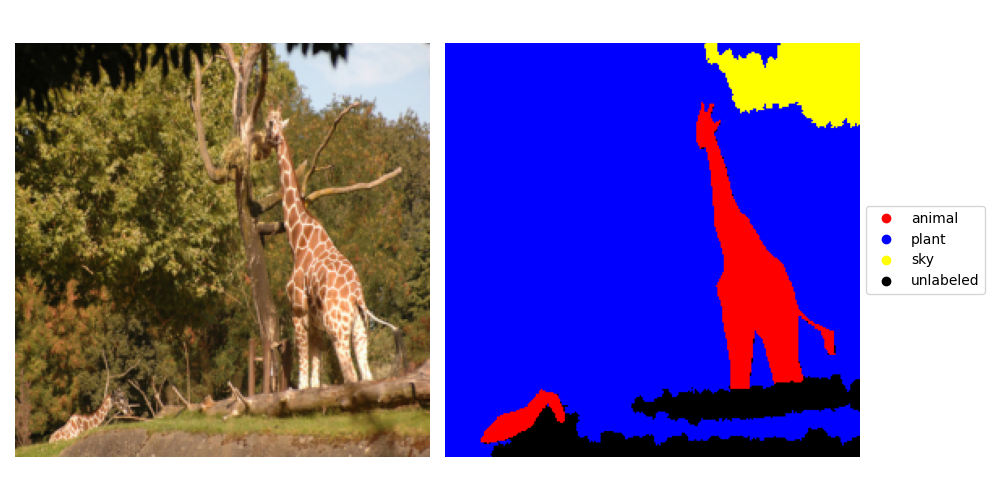
\includegraphics[width=0.5\textwidth]{figures/datasets/coco/samples/train/1.png}%
    }\\
    \subfloat[Validation sample 0]{%
        
\includegraphics[width=0.5\textwidth]{figures/datasets/coco/samples/val/0.png}%
    }
    \subfloat[Validation sample 1]{%
        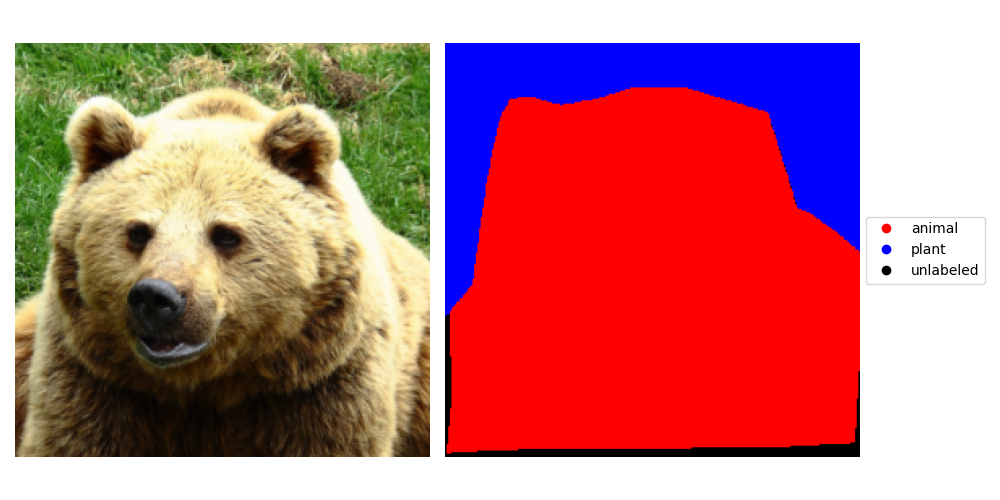
\includegraphics[width=0.5\textwidth]{figures/datasets/coco/samples/val/1.png}%
    }
    \caption{\label{fig:coco-samples}Ground truths for the dataset samples}
\end{figure}


\subsection{Training Settings}
All models are implemented in PyTorch~\cite{Ansel_PyTorch_2_Faster_2024} using an adapted version of the segmentation models repository~\cite{Iakubovskii:2019}. All code and configurations required to train the models and reproduce the experiments can be found on GitHub \footnote[1]{\url{https://github.com/Generative-AI-TUe/msc-project-1297333}}. All models are trained on a NVIDIA Geforce RTX 2080 TI. The gradients are clipped using the norm, with a maximum value of 10. The AdaMax~\cite{kingma2017adammethodstochasticoptimization} is used with a cosine annealing learning rate, varying between $1e^{-3}$ and $1e^{-4}$. Each model is trained on 10.000 minibatches of size 96 unless otherwise specified.

\section{Comparison to baseline architectures}
For the experiments we make use of our method, VAES (ours), FPN, and U-Net. Each model was trained eight times with different configurations. We used different settings for the pre-trained weights:
\begin{itemize}
    \item Without (`None') pre-trained weights.
    \item With pre-trained weights retrieved from the classification of ImageNet.
    \item With pre-trained weights retrieved from a $\beta$-vae, with $\beta=1$ and $\beta=100$.
\end{itemize}
Additionally, the model is trained with `frozen' encoder weights (the encoder weights are not updated), and with `unfrozen' encoder weights (the encoder weights are updated). The resulting Evaluation Jaccard Index can be seen in Table~\ref{tab:baseline_results}.

\begin{table}[ht]
\centering
\caption{The Evaluation Jaccard Index for our model and the baselines for various parameters. The higher the score, the better.}
\label{tab:baseline_results}
\begin{tabular}{llrrrr}
\toprule
 & weights & None & imagenet & vae-b1 & vae-b100 \\
frozen & architecture &  &  &  &  \\
\midrule
\multirow[t]{3}{*}{False} & VAES & 0.21 & 0.47 & 0.20 & 0.15 \\
 & fpn & \textbf{0.30} & \textbf{0.52} & \textbf{0.26} & \textbf{0.28} \\
 & unet & 0.23 & 0.49 & 0.21 & 0.24 \\
\cline{1-6}
\multirow[t]{3}{*}{True} & VAES & n.a. & 0.40 & 0.20 & 0.18 \\
 & fpn & n.a. & 0.45 & 0.21 & 0.21 \\
 & unet & n.a. & 0.42 & 0.20 & 0.19 \\
\cline{1-6}
\bottomrule
\end{tabular}
\end{table}


An Analysis of Variance (ANOVA) is done, of which the results can be seen in Table~\ref{tab:comparison_baselines_anova_all}. Based on these results an Ordinary Least Squares Linear Model (OLS) is fitted to determine the effect of each significant parameter. The results of this are shown in Table~\ref{tab:comparison_baselines_ols_effects}.

\begin{figure}[h]
    \foreach \i in {0,1,...,4} {
            \centering
            \subfloat[Image]{\includegraphics[width=0.2\textwidth]{figures/baselines/samples/VAES-imagenet-False/\i.png}}
            \subfloat[Ground Truth]{\includegraphics[width=0.2\textwidth]{figures/baselines/samples/VAES-imagenet-False/gt_\i.png}}
            \subfloat[VAES-imagenet]{\includegraphics[width=0.2\textwidth]{figures/baselines/samples/VAES-imagenet-False/pr_\i.png}}
            \subfloat[unet-imagenet]{\includegraphics[width=0.2\textwidth]{figures/baselines/samples/unet-imagenet-False/pr_\i.png}}
            \subfloat[fpn-imagenet]{\includegraphics[width=0.2\textwidth]{figures/baselines/samples/fpn-imagenet-False/pr_\i.png}}
            \\
        }
    \caption{Samples of the validation dataset, with the ground truth and the prediction by the model. The encoder is not frozen.}\label{ref:baseline-sample-results-0}
\end{figure}

\begin{table}[ht]
\centering
\caption{ANOVA results estimating the influence of each parameter.\\Where: \\\hphantom{tabb}`weights' are the pretrained weights (or lack thereof) used.\\\hphantom{tabb}`architecture' is the model architecture used.\\\hphantom{tabb}'frozen' indicates whether the encoder was frozen\\\hphantom{tabb}$A$:$B$ is the interaction effect between $A$ and $B$}
\label{tab:comparison_baselines_anova_all}
\begin{tabular}{lrrrrr}
\toprule
 & df & sum\_sq & mean\_sq & F & PR(>F) \\
\midrule
frozen & 1.00 & 0.00 & 0.00 & 5.29 & 0.08 \\
weights & 3.00 & 0.25 & 0.08 & 175.48 & \textbf{0.00} \\
architecture & 2.00 & 0.01 & 0.01 & 12.69 & \textbf{0.02} \\
frozen:weights & 3.00 & 0.00 & 0.00 & 1.53 & 0.34 \\
frozen:architecture & 2.00 & 0.00 & 0.00 & 2.16 & 0.23 \\
weights:architecture & 6.00 & 0.00 & 0.00 & 0.64 & 0.70 \\
Residual & 4.00 & 0.00 & 0.00 & n.a. & n.a. \\
\bottomrule
\end{tabular}
\end{table}


\begin{table}[ht]
\centering
\caption{Coefficients of the OLS showing the influence of the hyperparameters on the Evaluation Jaccard Index.\\Where:\\\hphantom{tabb}Coef. is the effectsize.\\\hphantom{tabb}P> |t| is the $p$-value. Bolded if significant ($\alpha\le0.05$).}
\label{tab:comparison_baselines_ols_effects}
\begin{tabular}{lrrrrrr}
\toprule
 & Coef. & Std.Err. & t & P>|t| & [0.025 & 0.975] \\
\midrule
Intercept & 0.22 & 0.02 & 10.54 & \textbf{0.00} & 0.17 & 0.26 \\
weights[T.imagenet] & 0.21 & 0.02 & 9.59 & \textbf{0.00} & 0.17 & 0.26 \\
weights[T.vae-b1] & -0.03 & 0.02 & -1.33 & 0.20 & -0.08 & 0.02 \\
weights[T.vae-b100] & -0.03 & 0.02 & -1.54 & 0.14 & -0.08 & 0.01 \\
architecture[T.fpn] & 0.06 & 0.02 & 3.49 & \textbf{0.00} & 0.02 & 0.09 \\
architecture[T.unet] & 0.02 & 0.02 & 1.48 & 0.16 & -0.01 & 0.06 \\
\bottomrule
\end{tabular}
\end{table}


\section{Reduction data required}
To determine if pre-training results in a reduction of labeled training data required, a full factorial design is done over the parameters: architecture type, pre-trained weights, and the percentage of the (labeled) dataset used. The resulting Evaluation Jaccard Index of each model configuration can be seen in Table~\ref{tab:data_fraction_results} and is plotted in Figure~\ref{fig:dataset-fraction-results}.
\begin{table}[ht]
\centering
\caption{The Evaluation Jaccard Index for the various models and dataset fractions. The higher the score the better.}
\label{tab:data_fraction_results}
\begin{tabular}{llrrrr}
\toprule
 & fraction & 1.000000 & 0.100000 & 0.010000 & 0.001000 \\
architecture & weights &  &  &  &  \\
\midrule
\multirow[c]{3}{*}{VAES} & None & 0.15 & 0.16 & 0.18 & 0.12 \\
 & imagenet & 0.34 & 0.37 & 0.39 & 0.21 \\
 & vae-b10 & 0.14 & 0.16 & 0.18 & 0.12 \\
\multirow[c]{3}{*}{fpn} & None & 0.22 & 0.12 & 0.21 & 0.17 \\
 & imagenet & 0.45 & \textbf{0.48} & \textbf{0.48} & \textbf{0.34} \\
 & vae-b10 & 0.19 & 0.21 & 0.23 & 0.16 \\
\multirow[c]{3}{*}{unet} & None & 0.21 & 0.10 & 0.18 & 0.14 \\
 & imagenet & \textbf{0.46} & 0.44 & 0.43 & 0.30 \\
 & vae-b10 & 0.20 & 0.18 & 0.21 & 0.14 \\
\bottomrule
\end{tabular}
\end{table}


\begin{figure}[h]
    \centering
    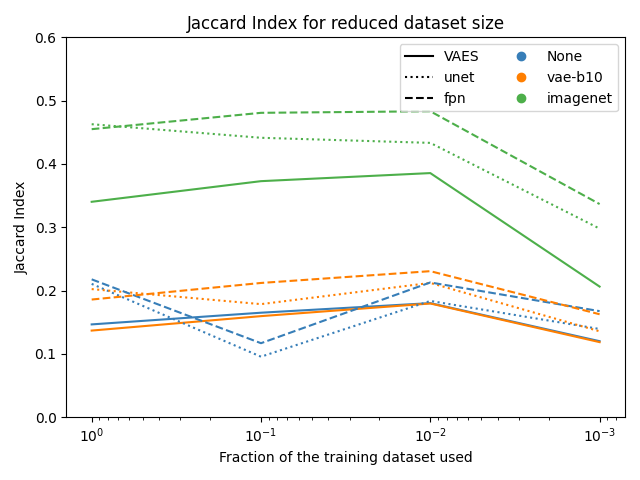
\includegraphics[width=0.9\textwidth]{figures/data_percentage/line-plot.png}
    \caption{Jaccard Index for reduced training dataset size.}
    \label{fig:dataset-fraction-results}
\end{figure}

An Analysis of Variance (ANOVA) is done, of which the results can be seen in Table~\ref{tab:data_fraction_parameter_significance}. Based on these results, it can be determined that there are no significant interaction effects between any of the parameters and that each individual parameter has a significant effect.
\begin{table}[ht]
\centering
\caption{Anova results estimating the influence of each parameter.\\Where: \\\hphantom{tabb}`weights' are the pretrained weights (or lack thereof) used.\\\hphantom{tabb}`architecture' is the model architecture used.\\\hphantom{tabb}`$\log_{10}(\text{fraction})$' is the fraction of data used in log scale.\\\hphantom{tabb}$A$:$B$ is the interaction effect between $A$ and $B$}
\label{tab:data_fraction_parameter_significance}
\begin{tabular}{lrrrrr}
\toprule
 & df & sum\_sq & mean\_sq & F & PR(>F) \\
\midrule
weights & 2.00 & 0.39 & 0.20 & 75.49 & \textbf{0.00} \\
architecture & 2.00 & 0.02 & 0.01 & 4.61 & \textbf{0.02} \\
weights:architecture & 4.00 & 0.01 & 0.00 & 0.93 & 0.47 \\
$\log_{10}(\text{fraction})$ & 1.00 & 0.02 & 0.02 & 6.45 & \textbf{0.02} \\
$\log_{10}(\text{fraction})$:weights & 2.00 & 0.01 & 0.01 & 2.11 & 0.15 \\
$\log_{10}(\text{fraction})$:architecture & 2.00 & 0.00 & 0.00 & 0.22 & 0.80 \\
$\log_{10}(\text{fraction})$:weights:architecture & 4.00 & 0.00 & 0.00 & 0.01 & 1.00 \\
Residual & 18.00 & 0.05 & 0.00 & n.a. & n.a. \\
\bottomrule
\end{tabular}
\end{table}


The effect of the parameters can then be analysed by a simple OLS model. The results of which are shown in Table~\ref{tab:data_fraction_parameter_influence}. It shows that there is a large and significant increase in performance when using the ImageNet weights. The weights gained from pre-training a VAE do not significantly affect the performance, compared to random weights. Furthermore, both the FPN and U-Net architectures are better than the VAES architecture. Finally, the size of the dataset is significant, however, it is more important to choose the right architecture and especially pre-trained weights.
\begin{table}
    \centering
    \caption{Coefficients of the OLS.\\Where:\\\hphantom{tabb}Coef. is the effectsize.\\\hphantom{tabb}P> |t| is the $p$-value. Bolded if significant ($\alpha\leq0.05$).}
    \label{tab:data_fraction_parameter_influence}
    \begin{tabular}{lrrrrrr}
        \toprule
                                     & Coef. & Std.Err. & t     & P>|t|         & [0.025 & 0.975] \\
        \midrule
        Intercept                    & 0.16  & 0.02     & 7.56  & \textbf{0.00} & 0.12   & 0.20   \\
        weights[T.imagenet]          & 0.23  & 0.02     & 11.66 & \textbf{0.00} & 0.19   & 0.27   \\
        weights[T.vae-b10]           & 0.01  & 0.02     & 0.67  & 0.50          & -0.03  & 0.05   \\
        architecture[T.fpn]          & 0.06  & 0.02     & 3.19  & \textbf{0.00} & 0.02   & 0.10   \\
        architecture[T.unet]         & 0.04  & 0.02     & 2.05  & \textbf{0.05} & 0.00   & 0.08   \\
        $\log_{10}(\text{fraction})$ & 0.02  & 0.01     & 2.71  & \textbf{0.01} & 0.00   & 0.03   \\
        \bottomrule
    \end{tabular}
\end{table}


\section{Model Characteristics}

As the computational resources in mobile robots tend to be low, the inference speed and memory usage were measured. Inference was done on a NVIDIA GTX 1070, and measured using PyTorch benchmarking tools. The results can be seen in Table~\ref{tab:model_characteristics}.

\begin{longtable}[ht]{lrrrrrrrrrr}
\caption{Characteristics of the various architectures with ResNet50 as backbone. Inference measurements were done on a NVIDIA GTX 1070.} \label{tab:model_characteristics} \\
\toprule
 & Parameters ($1e^6$) & Total MAC ($1e^9$) & \multicolumn{4}{r}{Inference Speed (ms)} & \multicolumn{4}{r}{Memory Usage (mb)} \\
 &   &   & 1 & 2 & 8 & 32 & 1 & 2 & 8 & 32 \\
Name &  &  &  &  &  &  &  &  &  &  \\
\midrule
\endfirsthead
\caption[]{Characteristics of the various architectures with ResNet50 as backbone. Inference measurements were done on a NVIDIA GTX 1070.} \\
\toprule
 & Parameters ($1e^6$) & Total MAC ($1e^9$) & \multicolumn{4}{r}{Inference Speed (ms)} & \multicolumn{4}{r}{Memory Usage (mb)} \\
 &   &   & 1 & 2 & 8 & 32 & 1 & 2 & 8 & 32 \\
Name &  &  &  &  &  &  &  &  &  &  \\
\midrule
\endhead
\midrule
\multicolumn{11}{r}{Continued on next page} \\
\midrule
\endfoot
\bottomrule
\endlastfoot
vaes & 82.70 & 5.28 & 15.71 & 14.87 & 28.46 & 70.84 & 755.95 & 760.34 & 779.35 & 1062.98 \\
unet & 32.52 & 2.72 & 10.20 & 10.02 & 16.71 & 49.66 & \textbf{549.91} & \textbf{554.11} & \textbf{579.54} & \textbf{770.77} \\
fpn & \textbf{26.12} & \textbf{1.95} & \textbf{9.57} & \textbf{9.65} & \textbf{15.44} & \textbf{47.06} & 602.86 & 606.14 & 634.45 & 904.72 \\
\end{longtable}



\section{Ablation Study}
\subsection{Backbone}
We first analyse the influence of the backbone on the performance of the VAE task by comparing the following backbones: MobileViT~\cite{Mehta2022SeparableSF}, MobileNetV2~\cite{sandler2019mobilenetv2invertedresidualslinear}, EfficientNet~\cite{tan2020efficientnetrethinkingmodelscaling}, and ResNet50~\cite{he2015deep}. The results can be seen in Table~\ref{tab:backbones-results}. Some examples of the reconstruction capabilities can be seen in Figure~\ref{fig:vae-backbones}.

\begin{figure}[!ht]
    \centering
    \caption{Example reconstruction for the various backbones.}
    \label{fig:vae-backbones}
    \subfloat[Original, EfficientNet]{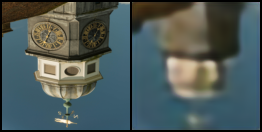
\includegraphics[width=0.45\linewidth]{figures/vae-backbones/samples/efficientnet_b2/4.png}}
    \subfloat[Original, MobileNetV2]{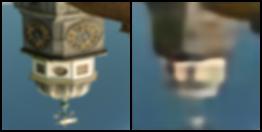
\includegraphics[width=0.45\linewidth]{figures/vae-backbones/samples/mobilenetv2_100/4.png}} \quad
    \subfloat[Original, MobileViT]{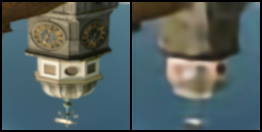
\includegraphics[width=0.45\linewidth]{figures/vae-backbones/samples/mobilevitv2_100/4.png}}
    \subfloat[Original, ResNet50]{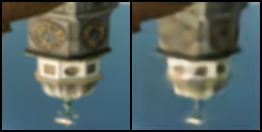
\includegraphics[width=0.45\linewidth]{figures/vae-backbones/samples/resnet50/4.png}}
\end{figure}

\begin{table}[ht]
\centering
\caption{VAE results of the various backbones.}
\label{tab:backbones-results}
\begin{tabular}{lrrrrr}
\toprule
 & Parameters ($1e^6$) & MAC ($1e^9$) & L1Loss (Recon) & KL-Divergence & Loss \\
Backbone &  &  &  &  &  \\
\midrule
MobileViT & 8.55 & 1.32 & 388158.31 & 5906.05 & 2402.00 \\
MobileNetV2 & \textbf{4.21} & \textbf{0.70} & 431505.41 & \textbf{5436.90} & 2774.02 \\
EfficientNet & 9.79 & 0.83 & 382322.31 & 16659.25 & 2911.08 \\
ResNet50 & 40.91 & 2.80 & \textbf{315560.38} & 9379.99 & \textbf{1792.29} \\
\bottomrule
\end{tabular}
\end{table}



\subsection{$\beta\text{-value}$}
We also analyse the effect of the $\beta$ factor on the reconstruction quality of the VAE. This is done by training models with varying values for $\beta$. The results can be seen in Table~\ref{tab:beta-vae-loss-values}. Some examples of the reconstruction capabilities can be seen in Figure~\ref{fig:beta-vae-recon-examples}. More samples can be seen in Appendix~\ref{appendix:recon_samples}.

\begin{table}[!ht]
    \centering
    \caption{Loss values resulting from training a Beta-VAE for various $\beta$ values}
    \label{tab:beta-vae-loss-values}
    \begin{tabular}{ccc}
        \hline
        $\beta$ & KL-Divergence & Reconstruction Error ($1e^5$) \\
        \hline
        0.01    & 80200         & 1.9                           \\
        0.1     & 31250         & 1.5                           \\
        1       & 8190          & 2.7                           \\
        10      & 2089          & 2.2                           \\
        100     & 498           & 2.9                           \\
        \hline
    \end{tabular}
\end{table}

\begin{figure}[!ht]
    \centering
    \caption{Example reconstructions for $\beta$-vae.}
    \label{fig:beta-vae-recon-examples}
    \subfloat[Original, $\beta$ = 0.01]{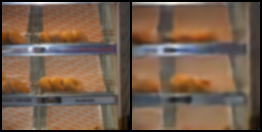
\includegraphics[width=0.45\linewidth]{figures/beta-vae/b0.01-0.png}}
    \subfloat[Original, $\beta$ = 0.1]{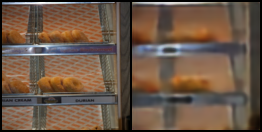
\includegraphics[width=0.45\linewidth]{figures/beta-vae/b0.1-0.png}} \quad
    \subfloat[Original, $\beta$ = 1]{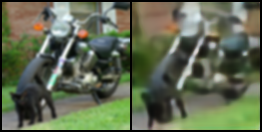
\includegraphics[width=0.45\linewidth]{figures/beta-vae/b1-0.png}}
    \subfloat[Original, $\beta$ = 10]{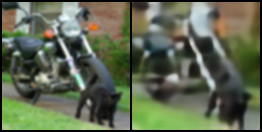
\includegraphics[width=0.45\linewidth]{figures/beta-vae/b10-0.png}}
\end{figure}


\subsection{Skip Connection}
To understand the importance of the type and amount of skip connections that are added after the pre-training, we will show the effect of this by incrementally removing more skip connections. We vary the amount of skip connections from 1 to 5 and try all 3 skip connection types. The results can be viewed in Table~\ref{tab:skip_results}.
Again an ANOVA is fitted to determine the significant effects, the results can be seen in Table~\ref{tab:skip_importance_anova_all}. Then, an OLS is fitted to show the effect size of all significant factors, the results of which can be seen in Table~\ref{tab:skip_importance_ols_effects}. From this limited sample of runs, the type does not seem to be significant. Neither does the amount of skip connections prove to be a significant effect based on the OLS. However, they are both close to a significance value of $0.05$, thus a bigger sample might show a small (likely positive) effect.

\begin{table}[ht]
\centering
\caption{Evaluation Jaccard Index for the VAES using different amounts and types of skip connections.}
\label{tab:skip_results}
\begin{tabular}{llrrr}
\toprule
 & skip\_type & proj & skip & var \\
 & skip\_num &  &  &  \\
\midrule
\multirow[c]{5}{*}{Evaluation Jaccard Index} & 1 & 0.412 & \textbf{0.426} & 0.410 \\
 & 2 & \textbf{0.462} & 0.452 & 0.429 \\
 & 3 & 0.474 & \textbf{0.493} & 0.463 \\
 & 4 & 0.456 & \textbf{0.494} & 0.434 \\
 & 5 & 0.440 & \textbf{0.490} & 0.433 \\
\multirow[c]{5}{*}{Parameters (x$1e^6$)} & 1 & 70.275 & \textbf{32.525} & 108.026 \\
 & 2 & 79.714 & \textbf{32.525} & 126.903 \\
 & 3 & 82.073 & \textbf{32.525} & 131.622 \\
 & 4 & 82.663 & \textbf{32.525} & 132.802 \\
 & 5 & 82.700 & \textbf{32.525} & 132.876 \\
\multirow[c]{5}{*}{Total MAC (x$1e^9$)} & 1 & 3.319 & \textbf{2.715} & 3.923 \\
 & 2 & 3.923 & \textbf{2.715} & 5.131 \\
 & 3 & 4.527 & \textbf{2.715} & 6.340 \\
 & 4 & 5.132 & \textbf{2.715} & 7.548 \\
 & 5 & 5.283 & \textbf{2.715} & 7.851 \\
\bottomrule
\end{tabular}
\end{table}


\begin{table}[ht]
\centering
\caption{ANOVA results estimating the influence of each parameter.\\Where: \\\hphantom{tabb}`weights' are the pretrained weights (or lack thereof) used.\\\hphantom{tabb}`architecture' is the model architecture used.\\\hphantom{tabb}'frozen' indicates whether the encoder was frozen\\\hphantom{tabb}$A$:$B$ is the interaction effect between $A$ and $B$}
\label{tab:comparison_baselines_anova_all}
\begin{tabular}{lrrrrr}
\toprule
 & df & sum\_sq & mean\_sq & F & PR(>F) \\
\midrule
frozen & 1.00 & 0.00 & 0.00 & 5.29 & 0.08 \\
weights & 3.00 & 0.25 & 0.08 & 175.48 & \textbf{0.00} \\
architecture & 2.00 & 0.01 & 0.01 & 12.69 & \textbf{0.02} \\
frozen:weights & 3.00 & 0.00 & 0.00 & 1.53 & 0.34 \\
frozen:architecture & 2.00 & 0.00 & 0.00 & 2.16 & 0.23 \\
weights:architecture & 6.00 & 0.00 & 0.00 & 0.64 & 0.70 \\
Residual & 4.00 & 0.00 & 0.00 & n.a. & n.a. \\
\bottomrule
\end{tabular}
\end{table}


\begin{table}[ht]
\centering
\caption{Coefficients of the OLS showing the influence of the hyperparameters on the Evaluation Jaccard Index.\\Where:\\\hphantom{tabb}Coef. is the effectsize.\\\hphantom{tabb}P> |t| is the $p$-value. Bolded if significant ($\alpha\le0.05$).}
\label{tab:comparison_baselines_ols_effects}
\begin{tabular}{lrrrrrr}
\toprule
 & Coef. & Std.Err. & t & P>|t| & [0.025 & 0.975] \\
\midrule
Intercept & 0.22 & 0.02 & 10.54 & \textbf{0.00} & 0.17 & 0.26 \\
weights[T.imagenet] & 0.21 & 0.02 & 9.59 & \textbf{0.00} & 0.17 & 0.26 \\
weights[T.vae-b1] & -0.03 & 0.02 & -1.33 & 0.20 & -0.08 & 0.02 \\
weights[T.vae-b100] & -0.03 & 0.02 & -1.54 & 0.14 & -0.08 & 0.01 \\
architecture[T.fpn] & 0.06 & 0.02 & 3.49 & \textbf{0.00} & 0.02 & 0.09 \\
architecture[T.unet] & 0.02 & 0.02 & 1.48 & 0.16 & -0.01 & 0.06 \\
\bottomrule
\end{tabular}
\end{table}

